\documentclass{article}

\usepackage{graphicx} %package to manage images
\graphicspath{ {images/} }

\usepackage[parfill]{parskip}
\usepackage[letterpaper, margin=1.2in]{geometry}
\usepackage[utf8]{inputenc}
\usepackage{setspace}
\doublespacing

\usepackage{hyperref}
\hypersetup{
    colorlinks=true,
    linkcolor=blue,
    filecolor=magenta,      
    urlcolor=blue,
}

\setlength{\parskip}{0em}

\title{Genetic Algorithm Applications}
\author{Penghuan Ni}
\date{April 2017}

\begin{document}

\maketitle

\section{Introduction}
We have learned the Genetic Algorithm(GA) in the class, but what applications does it have becomes a question in my mind. When we talk about other algorithms, such as K-means, we know it is a cluster algorithm, decision tree, we know it is a classifier, RNN, we know it is good at image recognition. However, when we talk about evolutionary algorithms, we usually do not have a clear picture about it. Based on this concern, I decide to do some research about GA applications. In my research, first, I will introduce some basic concept about Data Mining, Machine Learning(ML) and Multi-Objective Optimization(MOO). After that, I will introduce some applications about GA to give you a big picture about it. Then, I will talk about Premature Convergence problem in GA and give you a summary about using GA to solve ML problems. At the end, I will use GA to solve a problem to show you how to use it.

\section{Data Mining, Machine Learning and Multi-Objective Optimization}
Generally, data mining (sometimes called data or knowledge discovery) is the process of analyzing data from different perspectives and summarizing it into useful information. The aim of any data mining technique is to build an efficient predictive or descriptive model of a large amount of data. We have many tasks involved in data mining area, such as feature selection, classification, clustering, association rule mining, ensemble learning, etc. In my project, I will mainly focus on the first three tasks. \\

Another concept, which is so close to Data Mining, is Machine Learning. Machine learning focus more on algorithm part. Machine learning tasks are typically classified into three broad categories, supervised learning, unsupervised learning and reinforcement learning. We use ML learning algorithms to deal with data mining tasks. \\

The next concept involved in my project is Multi-Objective Optimization. In many real-word situations, there may be several objectives that must be optimized simultaneously in order to solve a certain problem. It is difficult to compare one solution with another one. In general, these problems admit multiple solutions, each of which is considered acceptable and equivalent when the relative importance of the objectives is unknown. However, the best solution is subjective and depends on the need of the designer or decision maker. In the past 30 years, researchers have come up with a couple of Multi-Objective Genetic Algorithms to use for different problems.

\section{Feature Selection}
Feature selection is one of the ML task. The goal of feature selection is to find an optimum relevant set of features or attributes that are necessary for the recognition process (classification or clustering). It helps us to deal with the high dimension data set. Usually, there are three reasons for us to do the feature selection: first, it is practically and computationally difficult to work with a large number of features. Second, many of those given features could be noisy, redundant and irrelevant to our task. Last, there will be a problem if we have more feature than the number of instances. Next, I will go through the step of using GA to solve Feature Selection task. \cite{survey1} \\

To apply GA on feature selection problem, we first need to come up with a way to representation each chromosome. In most of cases, binary encoding chromosome is enough for feature selection and it is widely used by people. The length of each chromosome is taken as d, where d is the total number of features. Each position of the chromosome can take either a 1 or 0 value. If position i has value 1, then the feature i has a value of part of the selected feature subset. If position i has a value of 0, then the corresponding feature is ignored. Then we can apply the GA operators on the chromosome. \\

For GA operators, since we are using the binary encoding, each chromosome is a binary string, the standard selection, crossover and mutation operators are enough. While, based on the length of your chromosome string, you may want to select different population size, mutation rate or other parameters. \\

After we know the chromosome representation and GA operators, the next thing we need to figure out is the objective functions (aka. fitness function). We use objective functions to evaluate each chromosome. Here we have two cases, supervised case and unsupervised case. For supervised case, we have training data and the feature selection task is usually about data classification. To evaluate each chromosome, we use some classification algorithms to measure the goodness of the selected feature subset based on how well they can classify the training examples using a certain classifier. Two objective functions we have for supervised case are reducing the misclassification rate as much as possible and minimize the size of feature set. For unsupervised case, we do not have training data and the feature selection task is usually about data clustering. To evaluate each chromosome, we use some clustering algorithms to measure the goodness of the feature subset on the basis of how well these features are able to identify the clustering structure of the data set. In this case, some cluster validity index is often used to evaluate the clustering result.

\section{Classification}
Classification is a ML supervised learning task. The goal of classification is to build a classifier from the training data. Through the classifier, we can assign each data point a class. There are mainly three different GA approaches we can take to do the classification task. The most commonly studied approach is the use of MOEAs for evolving a good set of classification rules. The second approach is to employ MOEAs to define the class boundaries (hyperplanes) in the training data. The final approach is to use MOEAs for training and model the construction of well known classifiers such as neural networks and decision tree classifiers. Next, I will briefly talk about those three approaches. \cite{survey1} \\

For Evolving Classification Rules approach, we usually representation a classification rule as a set of if-then rules, eg. If <condition> and <condition> and … Then <class>. For some continuous features, we need to discretized it before we use it as a classification rule. To make the chromosome, there are mainly two approaches. The first one is Pittsburgh approach, in which a set of rules is encoded in a single chromosome, which represent a complete classifier. The second one is the Michigan approach, where each chromosome encodes one rule and we need a set of rules to represent the classifier. For the objective function, we usually consider both accuracy and complexity of the candidate rule set.\\

For Evolving Class Boundaries (Hyperplanes) approach, we usually use GA to search a set of hyperplanes, which could separate the data. Also, in this case, we use binary chromosome to representation the parameter of those hyperplanes. By using this approach, three objectives are raised: minimize the number of misclassified patterns and the number of hyperplanes and maximize the classification accuracy.\\

For  Model Building of Standard Classifiers approach, we use GA to search the optimal parameters of the well known classifiers, such as ANN, SVM, and decision trees. In most case, we use binary to represent our chromosome. For different classifiers, we have different objective functions based on the classifier nature. There are three objectives for SVM, minimize the false positive rate, the false negative rate, and the number of support vectors. For RNN, we want to minimize the output error while minimizing the number of hidden units and the number of connections in order to reduce the complexity. Moreover, if we are building a decision tree, we want to maximize the classification accuracy and minimize the size of decision tree.

\section{Clustering}
Clustering is a ML unsupervised learning task. For unsupervised task, we do not have training data, which means we do not know the class or other criteria of each data. In unsupervised learning task, we are trying to find a suitable grouping of the dataset so that some criteria are optimized. Cluster validity index, which reflects the goodness of the clustering solutions, has been used to evaluate the clustering algorithm. Usually, there are three different cluster validity indices, external index, internal index and relative index. Multiobjective clustering techniques optimize more than one cluster validity index simultaneously.\cite{survey2} \\

There are mainly two chromosome representation approaches: prototype-based approach and point-based approach. The prototype-based approach encode the cluster centroids, medoids and modes into chromosome, while the point-based approach encode each instance’s cluster number into chromosome. Each of those two approaches have its own strength and shortness. We should select them based on the problem we are facing with.

\section{Premature Convergence}
Since I had this Premature Convergence problem in my thesis, I would like to make a whole section to talk about it. Premature convergence means the population (chromosome pool) converge to a local optimal before it converge to the global optimal. After this happened, due to the GA's nature, the next generation is superior to the previous generation, our chromosome pool will become nearly identical. Then, it will take a long time for GA to escape from this local optimal. How to deal with premature convergence becomes an important and difficult task. \cite{diversity} \\

After we know the reason for premature convergence is each individual in the population pool is too alike, so, we need to increase the diversity of population pool. The first and most easiest method is to make sure all the individual in our population pool are different. To make this happen, when we produce the next generation we can check if we have the same individual in it before we add a new one in. The second way is to add an exploration and exploitation trade off. Instead of using GA operators to produce all individual of next generation, we occasionally add a random chromosome into next generation. In addition, there are some other ways to deal with premature convergence, such as, increase the population size, use uniform crossover, etc. The two methods I introduced here are probably the easiest ones.

\section{Summary of Using GA to solve ML problem}
In this section, I will briefly talk about the procedure of using GA to solve the ML task. First, we should clear about that GA is a searching and optimization algorithm. So, to use GA to solve ML problem, we need first translate the ML task into a searching or optimization problem. There may be many ways to do this translation, you may need to compare them and select one. For example, when we talk about classification, there are three ways to use GA and you need to select one based on your situation. After you decided how to use GA to solve the ML task, then you need to know how to do chromosome encoding. The binary encoding is easy and widely used. There are some other encoding methods for us to choose as well, for example, gray encoding, value encoding, permutation encoding, etc. Based on the problem we are solving, we can choose different encoding method. Then, there are some other GA parameters and operators to decide as well. For GA parameters, we need to decide the population size, mutation probability, selective pressure, etc. For GA operators, we need to decide the selection type, crossover type, mutation type, etc. Different GA parameters or operators will give us a huge different performance. Usually, those parameters and operators are picked based on our knowledge about the ML task. Last, which is also the most important part is to deal with the Premature Convergence problem to improve your GA performance.\\

This is just a summary write by myself, there will be a lot more details you need to pay attention when you apply GA to solve a ML problem.

\section{Experiment}
I did two experiments and none of them is complicated. The first one is to use GA to find the target string and the second one is to use the GA to find the target image.

\subsection{String Experiment}
For the first experiment, user is asked to input a target string, then the GA runs and finds the target string. For example, if user input is “hello world!”, which is a 12 characters string, then GA will run and try to find the target string. I coded it in C++ and each chromosome is just a string type. My fitness function calculates the Hamming distance between two strings, find the difference between each characters in the string and take sum of them. So the objective is just to minimize the Hamming distance until it becomes to 0. In this experiment, the objective is linear, which means there is no local optimal. Because it is linear, it could converge and give us the target string very fast. Moreover, since each character have 128 possible values, the search space is length of string * 128, eg, the search space of “hello world!” will be 12 * 128 = 1536. The small search space also guarantees that the running time won’t be so long. \\

After some analysis of the problem, then I can talk about the GA variables and operators I use in the program. The population size is 100 and mutation probability is 0.01. I use tournament selection, single point crossover and flip bit mutation operators. For the tournament selection, instead of just select two and find the better one, I add a tournament size variable and use it to control selective pressure. For example, if the tournament size is 4, then I select 4 individuals from previous populations and the best one could survive to the next generation. Single point crossover is just find a random crossover point and exchange the gene. For flip bit mutation, I use a for loop to go through each character in the chromosome, generate a random number between 0 and 1 each time, compare it with the mutation probability. If the generated random number is smaller than the mutation probability, then change it to a random character again. \\

Following is some of the results and only the best string has been printed out for each iteration. The left side result shows the beginning of the evolving process and the right side result shows the end of evolving process. We can see that it converges to our target string at the end. Cause the search space is quite small, this experiment only takes 1 or 2 seconds.

\begin{figure}[h]
    \centering
    \begin{minipage}{0.45\textwidth}
        \centering
        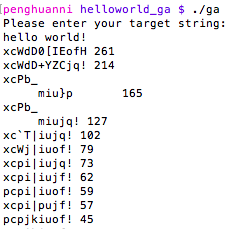
\includegraphics[width=0.9\textwidth]{hello1} % first figure
        \caption{String Experiment Result 1}
    \end{minipage}\hfill
    \begin{minipage}{0.45\textwidth}
        \centering
        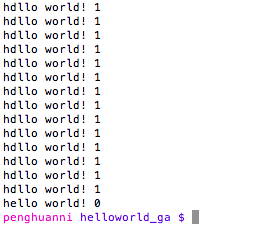
\includegraphics[width=0.9\textwidth]{hello2} % second figure
        \caption{String Experiment Result 2}
    \end{minipage}
\end{figure}


\subsection{Image Experiment}
For the second experiment, instead of using string as input, I use image as input. Since I do not have much experience with graphics in C++ before, I did a lot of research on it. There are many libraries we could use, such as OpenCV, ITK, OTB, CImg, etc. After some trial and error, I finally choose CImg. It is a small, open source image processing tookit for C++. You can find document, tutorial, and API under this link: \url{http://www.cimg.eu/}. \\

After I figure out the image processing, the rest of them becomes easier. I use each CImg object as a chromosome. Basically, each CImg object is just an integer vector, which value range is from 0 to 255. Since each pixel is using RGB color to represent, for a size of m by n image, the vector length is m*n*3*256. For example, if we have a 100*100 image, the CImg object will have 100*100*3*256 = 7680000 possible values. So, our search space has increased a lot. To deal with it, I did two things, increase the population size and decrease the mutation value. Since we want the chromosome with good gene could survive into next generation, I increase the tournament size as well. Even if I did some change to improve the performance, it still takes much longer time to converge.

Following is some images I generate from the beginning to the end of GA. The target image is a 100*100 image. First image is just randomly generated with random color values. Then the followings are generated by apply GA operators.

\begin{figure}[ht]
    \centering
    \begin{minipage}{0.45\textwidth}
        \centering
        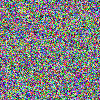
\includegraphics[width=0.8\textwidth]{bulldog000001} % first figure
        \caption{String Experiment Result 1}
    \end{minipage}\hfill
    \begin{minipage}{0.45\textwidth}
        \centering
        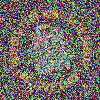
\includegraphics[width=0.8\textwidth]{bulldog000003} % second figure
        \caption{String Experiment Result 2}
    \end{minipage}
\end{figure}

\begin{figure}[ht]
    \centering
    \begin{minipage}{0.45\textwidth}
        \centering
        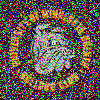
\includegraphics[width=0.8\textwidth]{bulldog000006} % first figure
        \caption{String Experiment Result 1}
    \end{minipage}\hfill
    \begin{minipage}{0.45\textwidth}
        \centering
        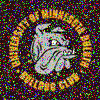
\includegraphics[width=0.8\textwidth]{bulldog000010} % second figure
        \caption{String Experiment Result 2}
    \end{minipage}
\end{figure}

\begin{figure}[ht]
    \centering
    \begin{minipage}{0.45\textwidth}
        \centering
        
\includegraphics[width=0.8\textwidth]{bulldog000015} % first figure
        \caption{String Experiment Result 1}
    \end{minipage}\hfill
    \begin{minipage}{0.45\textwidth}
        \centering
        
\includegraphics[width=0.8\textwidth]{bulldog000021} % second figure
        \caption{String Experiment Result 2}
    \end{minipage}
\end{figure}

\begin{figure}[ht]
    \centering
    \begin{minipage}{0.45\textwidth}
        \centering
        
\includegraphics[width=0.8\textwidth]{bulldog000028} % first figure
        \caption{String Experiment Result 1}
    \end{minipage}\hfill
    \begin{minipage}{0.45\textwidth}
        \centering
        
\includegraphics[width=0.8\textwidth]{bulldog} % second figure
        \caption{String Experiment Result 2}
    \end{minipage}
\end{figure}

Overall, through this experiment, I understand GA more, especially the GA parameters and GA operators.

\clearpage
%Sets the bibliography style to UNSRT and imports the 
%bibliography file "ref.bib".
\bibliographystyle{unsrt}
\bibliography{ref}

\end{document}
